\colorbox{green}{TEMPORARY - CM4}

\section{Deterministic Select}

In the previous part, we determine the Random Select algorithm in which we can find the $i^{th}$ smallest entry of an array T in $\Theta (n)$ (worst-case expected time). This algorithm was based on a variance of the quick sort.

The question asked is : Can we do it deterministic $\mathcal{O}(n)$ time?

To answer it, we must find a good pivot deterministically. This lead us to the following Deterministic Select (Code \ref{list:c4:deterministicselect}).

\begin{lstlisting}[label={list:c4:deterministicselect},caption=Pseudo-code of the Determinisic Select algorithm]
DeterministicSelect(T,i) :
    Split T into ceiling(n/5) arrays of maxsize = 5 
    
    foreach array : 
        find median % ceiling(n/5) medians = Theta(ceiling(n/5))
        
    Pivot = DeterminisiticSelect(medians, 1/2 * ceiling(n/5)) 
        % find the median of the medians computed
    
    Tlow = entries < pivot
    Thight = entries > pivot
    
    if (i <= |Tlow|)
        return DeterministicSelect(Tlow,i)
    if (i == |Tlow| + 1) 
        return pivot
    if (i > |Tlow| + 1)
        return DeterministicSelect(Thigh,i-|Tlow|-1)
\end{lstlisting}



Is this a good pivot?

As our pivot is the median of the different medians, we can say for sure that for the half of the array, the pivot is higher than the 3 smallest values (the median and the values smaller than the median). Thus we can affirm that the pivot is higher than at least $3\times \frac{1}{2} \times \ceil{\frac{n}{5}} \approx \frac{3n}{10}$.

We can do the same reasoning for the value higher than the pivot and also affirm that at least $3\times \frac{1}{2} \times \ceil{\frac{n}{5}} \approx \frac{3n}{10}$ values are higher for sure.

A simple drawing (Fig. \ref{fig:c4:deterministicselect}) can easily illustrate this reasoning.

\begin{figure}[!ht]
\centering
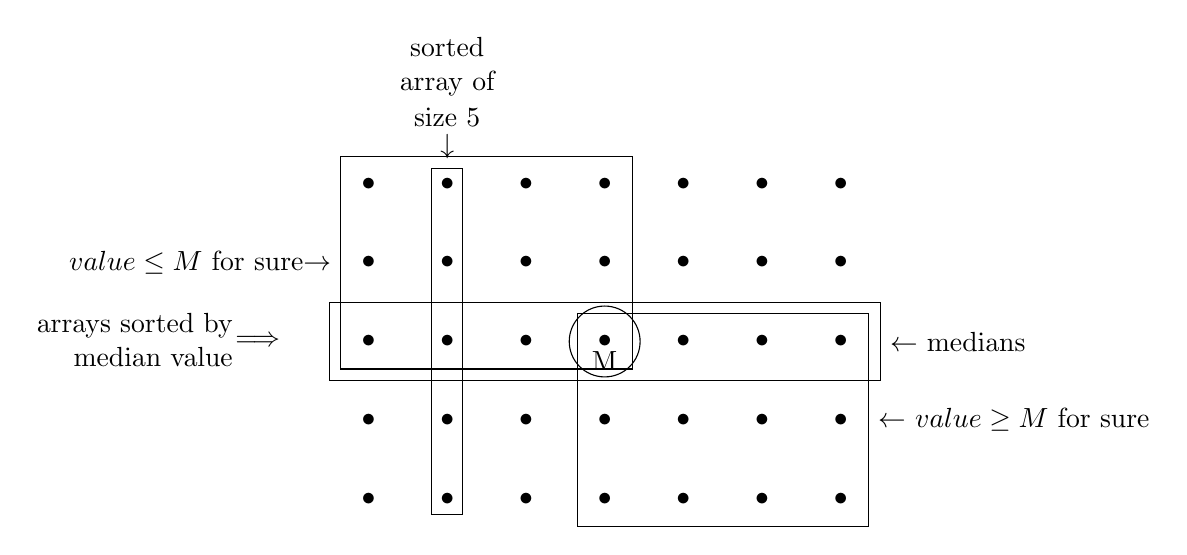
\begin{tikzpicture}
\draw (0,0) node {$\bullet$} ;
\draw (0,1) node {$\bullet$} ;
\draw (0,2) node {$\bullet$} ;
\draw (0,3) node {$\bullet$} ;
\draw (0,4) node {$\bullet$} ;
\draw (1,0) node {$\bullet$} ;
\draw (1,1) node {$\bullet$} ;
\draw (1,2) node {$\bullet$} ;
\draw (1,3) node {$\bullet$} ;
\draw (1,4) node {$\bullet$} ;
\draw (2,0) node {$\bullet$} ;
\draw (2,1) node {$\bullet$} ;
\draw (2,2) node {$\bullet$} ;
\draw (2,3) node {$\bullet$} ;
\draw (2,4) node {$\bullet$} ;
\draw (3,0) node {$\bullet$} ;
\draw (3,1) node {$\bullet$} ;
\draw (3,2) node {$\bullet$} ;
\draw (3,3) node {$\bullet$} ;
\draw (3,4) node {$\bullet$} ;
\draw (4,0) node {$\bullet$} ;
\draw (4,1) node {$\bullet$} ;
\draw (4,2) node {$\bullet$} ;
\draw (4,3) node {$\bullet$} ;
\draw (4,4) node {$\bullet$} ;
\draw (5,0) node {$\bullet$} ;
\draw (5,1) node {$\bullet$} ;
\draw (5,2) node {$\bullet$} ;
\draw (5,3) node {$\bullet$} ;
\draw (5,4) node {$\bullet$} ;
\draw (6,0) node {$\bullet$} ;
\draw (6,1) node {$\bullet$} ;
\draw (6,2) node {$\bullet$} ;
\draw (6,3) node {$\bullet$} ;
\draw (6,4) node {$\bullet$} ;
\draw (-1.6,2.2) node[left] {arrays sorted by};
\draw (-1.6,1.8) node[left] {median value};
\draw (-1,2) node[left] {$\Longrightarrow$};
\draw (0.8,-0.2) rectangle (1.2,4.2);
\draw (1,5.5) node[above]{sorted};
\draw (1,5) node[above]{array of};
\draw (1,4.6) node[above]{size 5};
\draw (1,4.2) node[above]{$\downarrow$};
\draw (-0.5,1.5) rectangle (6.5,2.5);
\draw (6.5,2) node[right]{$\leftarrow$ medians} ;
\draw (-0.35,4.35) rectangle (3.35,1.65);
\draw (-0.35,3) node[left]{$value \leq M$ for sure$\rightarrow$};
\draw (2.65,2.35) rectangle (6.35,-0.35);
\draw (6.35,1) node[right]{$\leftarrow$ $value \geq M$ for sure};
\draw (3,2) circle (0.45) ;
\draw (3,2) node[below]{M};
\end{tikzpicture}
\caption{Graphical view of the selection of the pivot (point M) in the \texttt{DeterministiSelect(T,i)}}
\label{fig:c4:deterministicselect}
\end{figure}

Knowing that, we can now compute the complexity of this algorithm by first writing down the recurrence equation :

\begin{align*}
t_n &= \underbrace{\Theta (n)}_{\text{split \& median finding}} + \underbrace{t_{\ent{n/5}}}_{\text{median of median}} + \underbrace{\Theta (n)}_{\text{split high low}} + \underbrace{\max \{ t_{|T_{low}|},1,t_{|T_{high}|} \}}_{\text{if cases}}\\ 
&\leq t_{n/5} + t_{7n/10} + \underbrace{\Theta (n)}_{f(n)}
\end{align*}

\begin{theorem}
$t_n = \mathcal{O} (n)$
\end{theorem}

\begin{proof}This will be proven by induction. By the hypothesis $f(n) = \Theta (n)$, we know that $f(n) \leq an$ (with $a>0$) for large enough $n$.

To be $\mathcal{O}(n)$, there must exist $c>0$ such as $t_n \leq cn$.

For $n$ small, the theorem is proven.

Now let's assume it is proven for $1,...,n-1$ and prove it for $n$ :

\begin{align*}
t_n &\leq t_{\frac{n}{5}} + t_{\frac{7n}{10}} + an\\
&\leq c \frac{n}{5} + c \frac{7n}{10} + an \\
&= c \frac{9n}{10} + an\\
&\leq cn &\text{if } a\leq \frac{1}{10}c
\end{align*}
\end{proof}


\chapter{Dynamic Programming}

\section{Computation of combinatorial value}



The goal is to compute the following combinatorial value  $$\tup{n}{k} = \frac{n!}{k!(n-k)!}$$

By definition, it can be computed by the following recurrence equation :

\begin{align*}
\tup{n}{k} &= \tup{n-1}{k-1} + \tup{n-1}{k} & \text{if } 0 < k<n\\
&=1 & \text{if } k=0\text{ or }n\\
&=0 & \text{otherwise}
\end{align*}

\subsection{Naive way : simple recursive algorithm}

A way to compute $\tup{n}{k}$ would be to follow the recurrence equation by using the following algorithm (List.\ref{list:c4:naive}).

\begin{lstlisting}[label={list:c4:naive},caption=Pseudo-code of the naive algorithm for the combinatorial]
C(n,k) :
    if (0 < k < n)
        return (C(n-1),k-1) + C(n-1,k))
    else if (k == 1 || k == n)
        return 1
    else
        return 0
\end{lstlisting}

It can be easily seen that this will lead to an enormous amount of recursive calls. The time complexity is thus a large number. But hopefully for us, there is redundancy in the computation! Some terms are computed many times. 

However, as the results are used directly in the computation, the space complexity is $\mathcal{O}(1)$.

\subsection{Better way using Pascal's triangle : "bottom-up" approach}

A better way is to store the intermediate result into a table : Pascal's triangle. We can build this table row by row.

As the computation of one term (knowing the recursive values) is done in $\Theta (1)$, the time complexity to fill the whole table is $\Theta (nk)$.

The space complexity is $\Theta (nk)$ if we keep all the intermediate values, but in fact we only need to keep one line at the same time, this reduce the space complexity to $\Theta (k)$.

If we compare the naive way with this one, we can see that the time complexity was improved at the expense of the space complexity. This effect is called the time-space trade-off.

This way of solving all the subproblem from the smallest to the final value (the one needed) is called the "bottom-up" approach.

\subsection{Third way with memoization : "top-down" approach} 

The "top-down" approach consist of taking the initial recursive algorithm and add a means of storing intermediate results.

We can for example use a table (initially set to $tab(n,k) = -1 \ \forall n,k$) and take the initial algo but before the computation, check if the result is already in the table. 

This is called recursive algorithm with memory function (or with memoization\footnote{if you doubt about the name, check out \url{http://en.wikipedia.org/wiki/Memoization}}). This technique can be useful for problems where we do not know in advance which subproblems are relevant and need to be computed because it compute exactly what's needed.

The time complexity will be the same as the bottom up approach ($\Theta (nk)$). But as we keep all intermediate result, we have a space complexity of $\Theta (nk)$. 

\section{Chained matrix multiplication}

\subsection{Choosing the execution order of the multiplications}

We want to compute the following matrix product : $ M = M_1M_2M_3...M_n$ with $M_i:d_{i-1}\times d_{i}$ matrix.

There exist several orders to proceed :
\begin{align*}
M&=(M_1M_2)(M_3M_4)\\
 &= ((M_1M_2)M_3)M_4\\ 
 &= M_1((M_2M_3)M_4)\\
 &=...
\end{align*}
Which order chose to minimise total computation time?

First let's compute the cost of multiplying 2 simple matrix (we neglect \bsc{Strassen} and all advance techniques,... we do the simple naive multiplication):\\
$cost(AB) = abc\text{ elementary multiplications}$ (if $A=a\times b$, $B=b\times c$ and thus $AB = a\times c$)

The order can matter: $cost((M_1M_2)M_3) = abc+acd = ac(b+d)$ and $cost(M_1(M_2M_3)) = bcd + abd=bd(c+a)$ (if $M_1=a\times b$, $M_2=b\times c$ and $M_3 = c\times d$).

How many possible orders for multiplying $n$ matrices?
The answer is $C_n = n^{th}$\bsc{Catalan} number
(from Eugène \bsc{Catalan}\footnote{\url{http://en.wikipedia.org/wiki/Eug\%C3\%A8ne_Charles_Catalan}}: 1814-1894 Belgium).

%%% mouais...
\begin{theorem}\label{cm4:valC}
Theorem :
\begin{align*}
C_0 &=0\\
C_1 &=1\\
C_n &= \sum_{i=1}^{n-1} C_iC_{n-i} = \sum_{i=0}^{n}C_iC_{n-i}
\end{align*}
\end{theorem}

\begin{proof} A simple proof of it can be made by looking at the following possibilities of decomposition of the product $M_1M_2..M_n$: 
$$\underbrace{(M_1)}_{C_1}\underbrace{(M_2..M_n)}_{C_{n-1}} || \underbrace{(M_1M_2)}_{C_2}\underbrace{(M_3..M_n)}_{C_{n-2}}|| ...|| \underbrace{(M_1..M_i)}_{C_i}\underbrace{(M_{i+1}..M_n)}_{C_{n-i}}|| ...|| \underbrace{(M_1..M_{n-1})}_{C_{n-1}}\underbrace{(M_n)}_{C_1}$$
\end{proof}



\begin{theorem}
$C_n = \frac{1}{n} \tup{2n-2}{n-1}$
\end{theorem}

\begin{proof}
The generating function\footnote{\url{http://fr.wikipedia.org/wiki/S\%C3\%A9rie_g\%C3\%A9n\%C3\%A9ratrice}} is $f(z) = \sum_{n\geq 0} C_n z^n = C_1z+C_2z^2 +...$

$f^2(z) = \sum_{n \geq 0}\sum_{i=0}^{n}C_i C_{n-i} z^n = C_1z^2+(C_1C_2+C_2C_1)z^3+....$ 

Because of the definition of $C_n$ at Theorem \ref{cm4:valC}, $f^2(z)=f(z) - z$ and $f^2(z)-f(z)+z = 0$.

By resolving the second degree equation, we found $f(z)=\frac{1\pm \sqrt{1-4z}}{2}$.

By Taylor's approximation ($\sqrt{1-4z}  = 1-2z-2z^2-...$). To have positive Taylor coefficients for $f(z)$ we should chose the solution with $-\sqrt{1-4z}$. We obtain $f(z) = \frac{1}{2}(1-\sqrt{1-4z}) = \frac{1}{2}(1-1+2z+2z^2+...) = \frac{1}{2}(2z+2z^2+...)$.

By the theorem \ref{cm4:newton}, we have
\begin{align*}
\sqrt{1-4z} &= (1-4z)^{1/2}\\
&= \sum_{i\geq 0} \tup{1/2}{i}(-4z)^i \underbrace{1^{1/2-i}}_{1}\\
&= \sum_{i\geq 0}\frac{(\frac{1}{2})!}{i!(\frac{1}{2} - i)!}(-4z)^i \underbrace{1^{1/2-i}}_{1}\\
&= \sum_{i\geq 0} \frac{\frac{1}{2}(\frac{-1}{2})(\frac{-3}{2}) ... (\frac{-(2i-3)}{2})}{i!} (-4z)^i
\end{align*}

By association of the coefficients, we get :
\begin{align*}
C_i &= \frac{-1}{2} \frac{(\frac{1}{2})(\frac{-1}{2})(\frac{-3}{2}) ... (\frac{-(2i-3)}{2})}{i!} (-1)^i 4^i\\
&=  \frac{1}{2}\frac{1}{2} \frac{\frac{1.3.5....(2i-3)}{2^{i-1}}}{i!}\frac{2.4.6...(2i-2)}{2.4.6...(2i-2)} 2^{2i} \\
&=\frac{(2i-2)!}{i!}\frac{1}{1.2.3...(i-1)}\frac{1}{4}\frac{1}{2^{i-1}}\frac{1}{2^{i-1}}2^{2i}\\
&=\frac{(2i-2)!}{i!(i-1)!} \\
&= \frac{1}{i}\frac{(2i-2)!}{(i-1)!(i-1)!}\\
&= \frac{1}{i}\tup{2i-2}{i-1}
\end{align*}

This implies that $$C_n = \frac{1}{n}\tup{2n-2}{n-1}$$
\end{proof}


\begin{theorem} \label{cm4:newton}
Newton binomial formula works also for $n\not\in \mathbb{N}$ : $$(x+y)^n = \sum_{i\geq 0} \tup{n}{i} x^i y^{n-i}$$
\end{theorem}

With \bsc{Stirling}'s approximation (
$n! \approx \left(\frac{n}{e}\right)^n \sqrt{2\pi n}$) we can obtain a more practical approximation of the order : 
\begin{align*}
C_n &= \frac{1}{n}\tup{2n-2}{n-1}\\
&= \frac{1}{n} \frac{(2n-2)!}{(n-1)!(n-1)!}\\
&\approx \frac{1}{n} \frac{\left(\frac{2n-2}{e}\right)^{2n-2} \sqrt{2\pi (2n-2)}}{\left(\frac{n-1}{e}\right)^{n-1} \sqrt{2\pi (n-1)}\left(\frac{n-1}{e}\right)^{n-1} \sqrt{2\pi (n-1)}}\\
&=\frac{1}{n} \frac{4^{n-1}\left(\frac{n-1}{e}\right)^{2n-2}\sqrt{4\pi}\sqrt{n-1}}{\left(\frac{n-1}{e}\right)^{2n-2}2\pi (n-1)}\\
&=\frac{4^n}{4\sqrt{\pi} n\sqrt{n-1}}\\
&= \Theta \left(\frac{4^n}{n^{3/2}}\right)
\end{align*}
This order is big due to the exponential component. There is no place for brute-force resolution (totally impractical)!
